\subsection{Technology stack}
To create and manage independent processing infrastructure we used Docker containers. This enables the application to run on different machines with different operating systems having Docker and Compose installed as the only requirement. 

The containers are started by Docker Compose. There is a driver container that launches Jupyter notebooks on \url{http://localhost:8888} and can run python notebooks with pynb. 

Jupyter notebook is an open-source tool for data science, that allows the users to execute scripts in an interactive fashion. It supports different programming languages and frameworks such as Python, R, pySpark and so on. It is mostly used for prototyping, since it is not suitable for clean and sustainable code with proper version control. Also it is not possible to automate running Jupyter notebooks as tasks. 
Pynb is a tool that allows to convert Jupyter notebooks to plain python code and vice verse. The maintenance of such python notebooks is more sustainable and it is possible to programatically run them. \cite{pynb}

The driver runs pySpark applications on the baseline standalone Spark cluster with one worker and one master with client deploy mode. In standalone cluster mode, Spark's own cluster manager is used instead of YARN or Mesos. Client deploy mode means that  the driver is launched in the same process as the client that submits the application. 

A master container that deploys Spark master, and a worker container that starts a worker with one core and 1 gigabyte of memory, connected to the master. The Spark web user interface shows the available worker on \url{http://localhost:8080}.

As a data-source we prefer Parquet over .csv, since most of the operations in the project involve iterating through all rows for given columns. This way we take advantage of the Parquet being an efficient columnar storage.

The project is written in Python 3 and it heavily utilizes the DataFrame API within Spark SQL. A DataFrame in pySpark is an immutable distributed collection of data. However, in contrast with an RDD, data is organized into named columns, akin to a table in a relational database, designed to make large data sets processing very easy.

We use Fabric to orchestrate the containers, run tests and execute tasks. It is more convenient to use a unified command line interface for recurring administration tasks. \cite{fabric}

\subsection{Data collection}
The following data sources are used:
\begin{itemize}
\item Cell map:
\begin{itemize}
    \item OpenCelliD public data set representing cell tower locations and meta data.
    \item Proprietary data set provided by Telefonica containing cell locations and meta data within the Telefonica Germany's cellular network.
\end{itemize}
\item CDR data: Sequences of mobile network events recorded on the test phone
\item GPS trajectories recorded on the test phone
\end{itemize}

\subsubsection{Cell map data set}
The full data set of OpenCelliD was downloaded as of 1 March 2018. The downloaded .csv file is 3.1 GB on disk. The following attributes of OpenCelliD data set are used for the analysis \cite{opencellid}:
\begin{itemize}
\item radio: \textit{string} - Network type. One of the strings GSM, UMTS, LTE or CDMA.
\item mcc:  \textit{integer}  -  Mobile Country Code, for example 262 for Germany.
\item net: \textit{integer} - For GSM, UMTS and LTE networks, this is the Mobile Network Code (MNC). For CDMA networks, this is the System Identification number (SID).
\item cell: \textit{integer} - Cell ID (CID) for GSM and LTE networks. UTRAN Cell ID / LCID for UMTS networks, which is the concatenation of 2 or 4 bytes of Radio Network Controller (RNC) code and 4 bytes of Cell ID. Base station identifier number (BID) for CDMA networks.
\item lat: \textit{double} - Latitude in degrees between -90.0 and 90.0.
\item lon: \textit{double} - Longitude in degrees between -180.0 and 180.0.
\item samples: \textit{integer} - Total number of measurements assigned to the cell tower.
\item changeable:  \textit{integer} - Defines if coordinates of the cell tower are exact or approximate. \footnote{changeable=1: the GPS position of the cell tower has been calculated from all available measurements. changeable=0: the GPS position of the cell tower is precise - no measurements have been used to calculate it.}
\item created: \textit{integer} - The first time when the cell tower was seen and added to the OpenCelliD database. \footnote{A date in time stamp format: number of seconds since the UTC Unix Epoch of 1970-01-01T00:00:00Z (For example 1409522613 is the time stamp for 2014-08-31T22:03:33Z).}
\item updated: \textit{integer} - The last time when the cell tower was seen and updated.
\end{itemize}

The other cell map data set used in the analysis is proprietary and therefore will not be discussed in details. It contains similar fields to the OpenCelliD cell map including location information and cell identification required for the analysis.

We expect less cell towers in the outskirts of the city and more towards the center. Figure \ref{fig:opencellid}\footnote{Only the latest observations are shown.} shows that the density of cell towers within Telfonica network from OpenCelliD is quite dense even in the outer regions of Berlin. Thus the data from OpenCelliD might be corrupted or of poor quality. In contrast Figure \ref{fig:tefnext} - showing the cell towers from the internal Telefonica cell map -  seems more reasonable and in line with our expectations.

\begin{figure}[h]
    \begin{minipage}[b]{0.5\textwidth}
    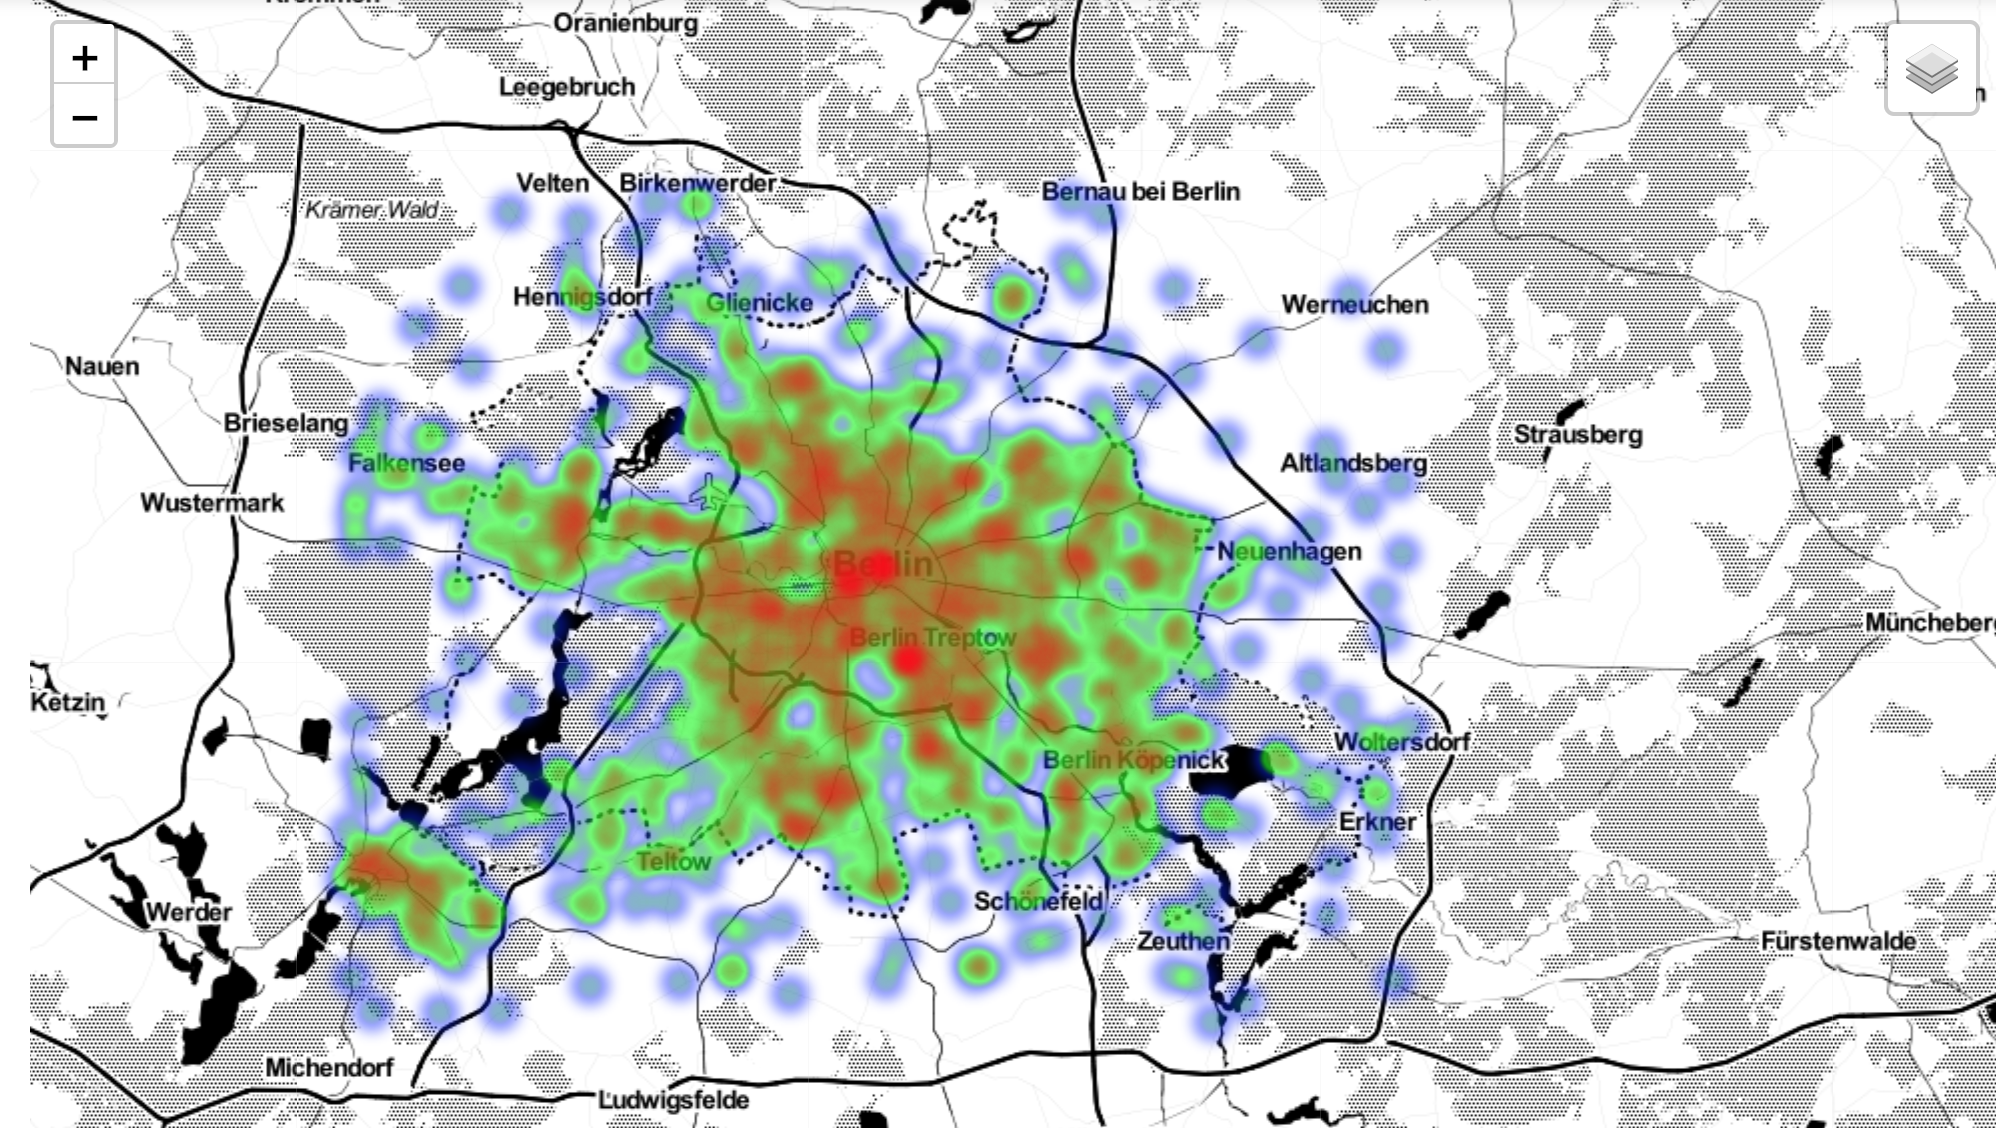
\includegraphics[width=\textwidth]{images/tefnext.png}
    \caption{Heatmap of Telefonica cell towers in Berlin (Source: Telefonica cell map data)}
    \label{fig:tefnext}

    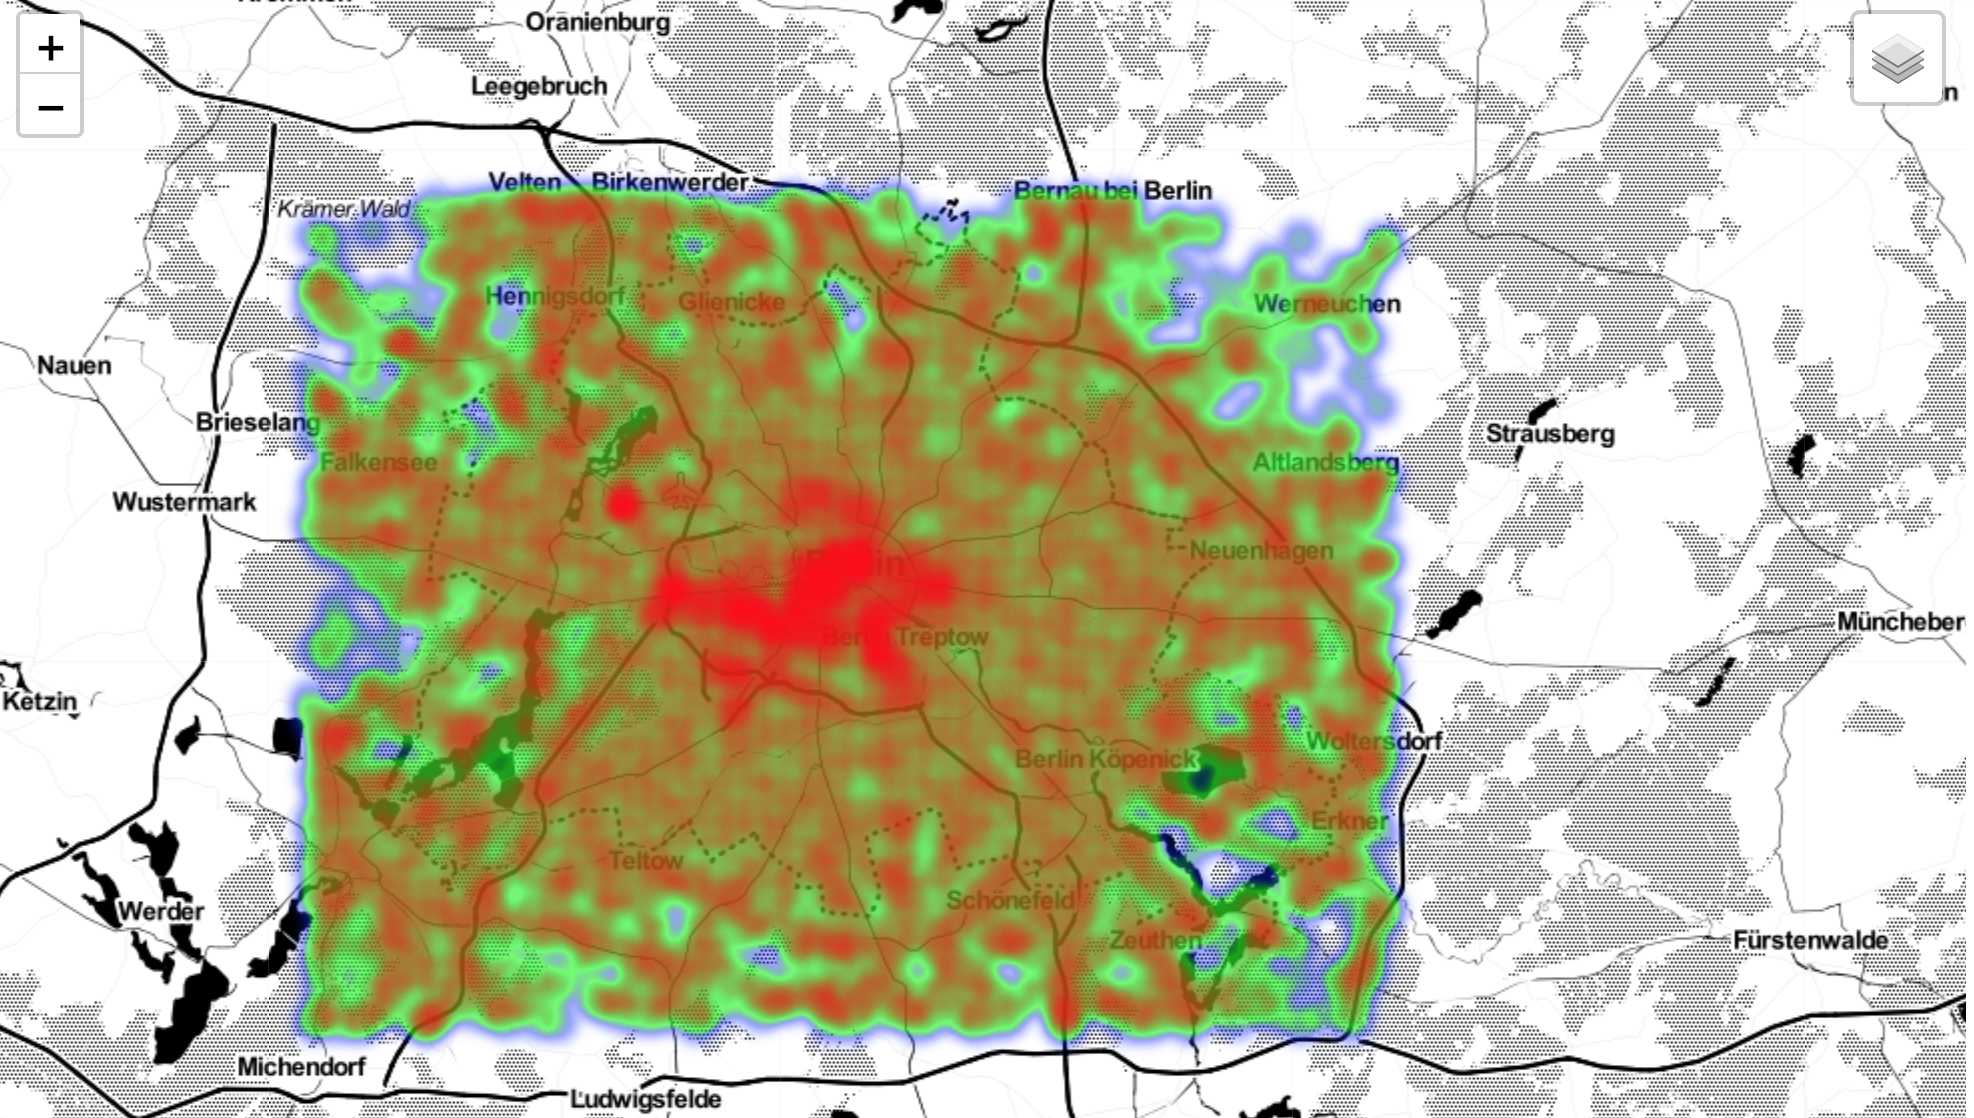
\includegraphics[width=\textwidth]{images/opencellid.png}
    \caption{Heatmap of Telefonica cell towers in Berlin (Source: OpenCelliD) }
    \label{fig:opencellid}
    \end{minipage}\qquad
\end{figure}

\subsubsection{CDR data}
The mobile network event data set generated between \date{2018/02/14} and \date{2018/02/21} in Berlin region with Nexus 4 E960 test phone (Android operating system) includes among others:
\begin{itemize}
\item unix\_ts: \textit{integer} - Date and time when event was generated in timestamp format, i.e. the number of seconds since Jan 01 1970. (UTC)
\item unix\_dt: \textit{datetime} - Date and time when event was generated.
\item event\_type: \textit{integer} - Integer code for type of the event.
\item network\_type: \textit{integer} - Integer code for type of the network.
\item lac: \textit{integer} - Location Area Code of the cell.
\item sac: \textit{integer} - Cell id.
\item source: \textit{string} - Packet type.
\end{itemize}

During data collection phase 666 CDR events were generated and collected by a user. There are cell towers that were assigned to the collected events more frequently than others. The 10 most frequently used cells are shown in Figure \ref{fig:freq_cells}. These are likely to be around the home or workplace of the user generating the data.

\begin{figure}[h]
    \centering
    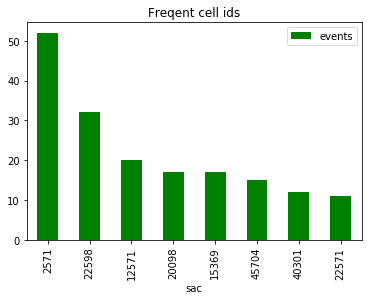
\includegraphics[width=0.5\textwidth]{images/frequent_cell_ids.png}
    \caption{Most frequently connected cell towers}
    \label{fig:freq_cells}
\end{figure}

On average there was a CDR event in about every five to ten minutes during the data collection. However that can be less frequent, depending on individual mobile usage preferences. 

\subsubsection{GPS trajectories data}
The GPS trace data set has the following columns:
\begin{itemize}
\item unix\_dt: \textit{datetime} - Date and time in Coordinated Universal Time (UTC).
\item lat: \textit{double} - Latitude in decimal degrees between -90.0 and 90.0.
\item lon: \textit{double} - Longitude in decimal degrees between -180.0 and 180.0.
\item accuracy: \textit{double} - Accuracy of measurement in meters.
\item satellites: \textit{integer} -  Number of reachable GPS satellites.
\end{itemize}

The traces were recorded for the same time-frame in Berlin area on the same test phone as the CDR events with GPSLogger Android application using the following specifications:
\begin{itemize}
\item Logging interval: 15 sec
\item Accuracy filter: 15m
\item Location provider: GPS
\item Logfile format: .csv and GeoJSON
\item On new trip: create new file
\item Timezone: UTC
\item Spatial reference system: WGS84
\end{itemize}

There are GPS observations in every one to three minutes therefore the GPS data is more dense compared to the CDR vents. 

\subsection{Data processing}\label{sec:data-proc}
The data-flow throughout the implementation steps can be seen on Figure \ref{fig:data-flow}.
\begin{figure}[h]
    \centering
    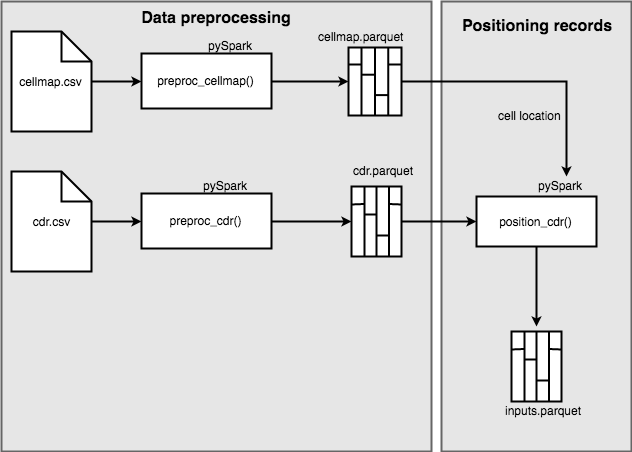
\includegraphics[width=0.5\textwidth]{images/data-flow.png}
    \caption{Data flow}
    \label{fig:data-flow}
\end{figure}

\subsubsection{Data pre-processing}
The cell map files cannot be fit into memory, therefore pySpark is used for the cleaning process with the following steps: 
\begin{enumerate}
    \item Import csv to pySpark DataFrame
    \item Drop irrelevant columns
    \item Keep only the records of cells in the Telefonica network in Berlin
    \item Write cleaned data to parquet files
\end{enumerate}

The raw GPS traces data set consists of several csv files, each trajectory having its own file. The data set is relatively small, however it is still processed using pySpark for future scalability. The cleaning process consists of the following steps: 
\begin{enumerate}
    \item Import .csv files to pySpark DataFrame
    \item Clean data:
    \begin{itemize}
        \item Create $trip\_id$ column from file name
        \item Change timezone of the timestamp
        \item Add unix\_ts timestamp column
        \item Drop irrelevant columns
        \item Drop rows where relevant columns are missing
    \end{itemize}
    \item Validate data quality.Check if: 
     \begin{itemize}
        \item columns changed in the input
        \item dates are in scope
        \item latitude and longitude values are valid
        \item data contains records from only one provider
    \end{itemize}
    \item If data quality is good, write cleaned data to Parquet files
\end{enumerate}

The CDR data-set generated by the test phone in the given time period is stored in a single .csv file. The size of the file is small, given only one device was used to record events for about one week. However the size of mobile network events generated daily can go up to hundreds of gigabytes per day. The following steps are executed during the cleaning process: 
\begin{enumerate}
   \item Import .csv files to pySpark DataFrame
    \item Clean data:
    \begin{itemize}
        \item Drop irrelevant columns
        \item Drop rows where relevant columns are missing
    \end{itemize}
    \item Validate data quality.Check if: 
    \begin{itemize}
        \item columns changed in the input
        \item dates are in scope
        \item event types are valid
    \end{itemize}
    \item If data quality is good, write cleaned data to Parquet files
\end{enumerate}

The DataFrames are re-partitioned before writing them to Parquet files to avoid having hundreds of tiny files for a relatively small data. 

\subsubsection{Positioning mobile network events}
Having preprocessed the raw data, the next step is to assign a location to each of the events in the CDR data-set from the cell map data-set based on the respective cell tower id. 
These steps are executed for positioning the CDR data:
\begin{itemize}
    \item Load CDR data from parquet files to pySpark DataFrame
    \item Load cell map data to pySpark DataFrame
    \item Prepare imported DataFrames
    \item Join CDR and cell map data-sets on cell id or ident (SAC and LAC)
    \item Persist joined DataFrame to parquet files
\end{itemize}

Events in the CDR data might be active or passive. Active events originate from the mobile device and passive events originate from the network. The cell id of active events are in general correct and can be trusted. The cell id of passive events represent the guess of the network and might provide erroneous information. Therefore positioning of passive events is prone to higher inaccuracy. 


\subsubsection{Merging mobile network events and GPS data set}
After positioning the records of the CDR data, we need to find the ground truth location for the given event. In other words, given a mobile network event, we match the closest point in GPS trace data considering the time stamps. The identified GPS point is then used as ground truth location for the mobile network event.

The following steps are taken:
\begin{itemize}
    \item Load CDR and GPS data-sets from parquet files to pySpark DataFrame
    \item Prepare DataFrames for join
    \item Join DataFrames on timestamp:
    \begin{itemize}
        \item Cross join two DataFrames
        \item Calculate difference between timestamp of GPS and CDR in each row
        \item Group by event id of CDR data
        \item For each group keep only one row that has the minimum difference in terms of time stamps
    \end{itemize}
\end{itemize}

